\section{Ускорение точек твёрдого тела в плоском движении}

Имеем согласно \ref{eq:figure_velocity}
\begin{equation*}
  \vec{v} = \vec{v}_0 + \crossprod{\vec{\omega}}{\pvec{r}}
\end{equation*}
и, следовательно,
\begin{equation*}
  \begin{aligned}
    \vec{w} &= \dt[\vec{v}] \\
    &= \dt[\vec{v}_0] + \dt
      (\crossprod{\vec{\omega}}{\pvec{r}}) \\
    &= \dt[\vec{v}_0] + \crossprod{\dt[\vec{\omega}]}{\pvec{r}} +
      \crossprod{\vec{\omega}}{\dt[\pvec{r}]}.
  \end{aligned}
\end{equation*}

Первое слагаемое
\begin{equation}
  \label{eq:translational_acceleration}
  \vec{w}_0 = \dt[\vec{v}_0],
\end{equation}
одинаковое для всех точек фигуры и равное ускорению полюса $O'$, называется
\textit{поступательным ускорением}.

Второе слагаемое --- обозначим его через $\vec{w}^\text{(в)}$, --- равное
\begin{equation}
  \label{eq:rotational_acceleration}
  \vec{w}^\text{(в)} = \crossprod{\dt[\vec{\omega}]}{\pvec{r}} =
    \crossprod{\vec{\varepsilon}}{\pvec{r}},
\end{equation}
называется \textit{вращательным ускорением}. Здесь вектор
\begin{equation*}
  \vec{\varepsilon} = \dt[\vec{\omega}]
\end{equation*}
представляет собой \textit{вектор углового ускорения}. Вектор
$\vec{w}^\text{(в)}$ перпендикулярен к $\pvec{r}$ и направлен в ту же сторону,
что и вращательная скорость $\crossprod{\vec{\omega}}{\pvec{r}}$ точки плоской
фигуры вокруг полюса, или в противоположную, сообразно тому, будет ли вращение
фигуры ускоренным или замедленным; величина $\vec{w}^\text{(в)}$ равна
\begin{equation*}
  w^\text{(в)} = \varepsilon r' \sin(\widehat{\vec{\varepsilon}, \pvec{r}}) =
    \varepsilon r'.
\end{equation*}

Третье слагаемое, которое обозначим $\vec{w}^\text{(ос)}$, равно
\begin{equation}
  \label{eq:centripetal_acceleration}
  \vec{w}^\text{(ос)} = \crossprod{\vec{\omega}}{\dt[\pvec{r}]}.
\end{equation}
Подставив сюда вместо $\dt[\pvec{r}]$ его значение \ref{eq:rotational_velocity},
получим
\begin{equation*}
  \vec{w}^\text{(ос)} = \crossprod{\vec{\omega}}
    {\crossprod{\vec{\omega}}{\pvec{r}}},
\end{equation*}
или, по известной формуле разложения двойного векторного произведения:
\begin{equation*}
  \vec{w}^\text{(ос)} = \vec{\omega} (\dotprod{\vec{\omega}}{\pvec{r}}) -
  \pvec{r} (\dotprod{\vec{\omega}}{\vec{\omega}}).
\end{equation*}
Но в плоском движении векторы $\vec{\omega}$ и $\pvec{r}$ взаимно
перпендикулярны, так что
\begin{equation*}
  \dotprod{\vec{\omega}}{\pvec{r}} = 0,
\end{equation*}
кроме того,
\begin{equation*}
  \dotprod{\vec{\omega}}{\vec{\omega}} = \omega^2,
\end{equation*}
следовательно,
\begin{equation*}
  \vec{w}^\text{(ос)} = -\omega^2 \pvec{r}.
\end{equation*}
Эта составляющая ускорения, направленная от рассматриваемой точки к полюсу и
равная по величине $\omega^2 r'$, называется \textit{осестремительным
ускорением}.

Итак, имеем
\begin{equation*}
  \label{eq:flat_motion_acceleration}
  \begin{aligned}
    \vec{w} &= \vec{w}_0 + \vec{w}^\text{(в)} + \vec{w}^\text{(ос)} \\
    &= \vec{w}_0 + \crossprod{\vec{\varepsilon}}{\pvec{r}} - \omega^2 \pvec{r},
  \end{aligned}
\end{equation*}
то есть ускорение любой точки в плоском движении может быть представлено как
геометрическая сумма поступательного ускорения, равного ускорению полюса,
вращательного ускорения вокруг полюса и осестремительного ускорения к полюсу.

Составим формулы для \textit{проекций ускорения на неподвижные оси} $x,~y$.
Замечая, что
\begin{equation*}
  \pvec{r} = \vec{r} - \vec{r}_0,
\end{equation*}
найдём, проектируя обе части равенства \ref{eq:flat_motion_acceleration} на
неподвижные оси $x$ и $y$:
\begin{equation}
  \label{eq:flat_acceleration_immovable_projections}
  \begin{gathered}
    w_x = \ddot{x}_0 - \ddot{\varphi} (y - y_0) - \dot{\varphi}^2 (x - x_0), \\
    w_y = \ddot{y}_0 + \ddot{\varphi} (x - x_0) - \dot{\varphi}^2 (y - y_0).
  \end{gathered}
\end{equation}

Аналогично найдём \textit{проекции ускорения на подвижные оси}:
\begin{equation}
  \label{eq:flat_acceleration_movable_projections}
  \begin{gathered}
    w_{x'} = w_{0x'} - \ddot{\varphi} y' - \dot{\varphi}^2 x', \\
    w_{y'} = w_{0y'} + \ddot{\varphi} x' - \dot{\varphi}^2 y'.
  \end{gathered}
\end{equation}

Условимся в дальнейшем снабжать обозначение ускорения индексом, указывающим
точку, ускорение которой рассматривается. Положим
\begin{equation*}
  \vec{w}_{AB} = \crossprod{\vec{\varepsilon}}{\pvec{r}_{AB}} - \omega^2
    \pvec{r}_{AB}.
\end{equation*}
Здесь вектор $\vec{w}_{AB}$ есть ускорение точки $B$ по отношению к точке $A$,
то есть ускорение по отношению к системе координат, имеющей начало в точке $A$ и
движущейся вместе с этой точкой поступательно. Вращательное ускорение вокруг
полюса и осестремительное ускорение к полюсу будем обозначать так:
\begin{equation*}
  \vec{w}_{AB}^\text{(в)} = \crossprod{\vec{\varepsilon}}{\pvec{r}_{AB}}, \quad
  \vec{w}_{AB}^\text{(ос)} = - \omega^2 \pvec{r}_{AB}.
\end{equation*}

Формула \ref{eq:flat_motion_acceleration} примет вид
\begin{equation}
  \label{eq:flat_motion_acceleration_named}
  \vec{w}_B = \vec{w}_A + \vec{w}_{AB} =
    \vec{w}_A + \vec{w}_{AB}^\text{(в)} + \vec{w}_{AB}^\text{(ос)}.
\end{equation}

Замечая, что $\vec{w}_{AB}^\text{(в)}$ и $\vec{w}_{AB}^\text{(ос)}$ взаимно
перпендикулярны, получим
\begin{equation}
  \label{eq:w_ab_length}
  w_{AB} = \pvec{r}_{AB} \sqrt{\varepsilon^2 + \omega^4}.
\end{equation}

Обозначим через $\pi - \alpha$ тупой угол, образуемый векторами $\pvec{r}_{AB}$
и $\vec{w}_{AB}$. Тогда
\begin{equation}
  \label{eq:instantaneous_acceleration_center_angle}
  \tg \alpha = \frac{\vec{w}_{AB}^\text{(в)}}{\vec{w}_{AB}^\text{(ос)}} =
    \frac{\tilde{\varepsilon}}{\omega^2}.
\end{equation}

\begin{theorem}
  В любой момент времени существует точка $Q$ плоской фигуры, ускорение которой
  в этот момент равно нулю.
\end{theorem}

\begin{proof}
  \begin{figure}[H]
    \centering
    \resizebox{\linewidth}{!}{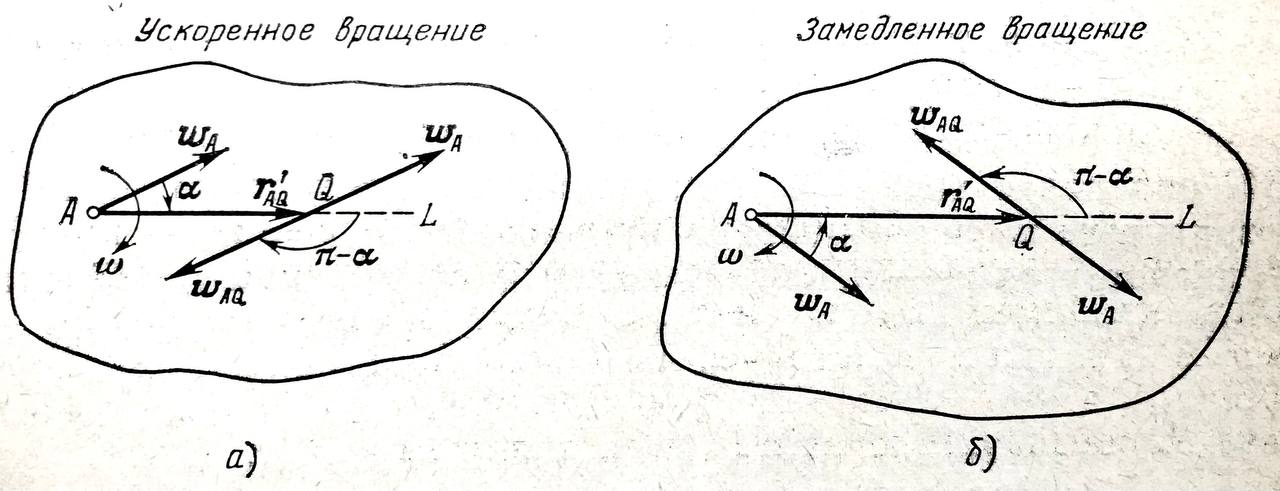
\includegraphics{src/mechanics/pictures/18_1.jpg}}

    \caption{}
    \label{fig:18_1}
  \end{figure}

  Проведём через какую-нибудь точку $A$ полупрямую $AL$ под углом $\alpha$,
  определяемым по формуле \ref{eq:instantaneous_acceleration_center_angle}, к
  вектору $\vec{w}_A$, отсчитывая $\alpha$ от $\vec{w}_A$ в сторону вращения
  фигуры или противоположно ему, сообразно тому, будет ли вращение ускоренным
  или замедленным. Отложим на $AL$ отрезок
  \begin{equation}
    \label{eq:instantaneous_acceleration_center_distance}
    r_{AQ}' = AQ = \frac{w_A}{\sqrt{\varepsilon^2 + \omega^4}}.
  \end{equation}
  Конец $Q$ этого отрезка и будет мгновенным центром ускорений. В самом деле,
  согласно формуле \ref{eq:w_ab_length} имеем
  \begin{equation*}
    w_{AQ} = r_{AQ}' \sqrt{\varepsilon^2 + \omega^4} = w_A.
  \end{equation*}
  С другой стороны, по построению вектор $\vec{w}_{AQ}$ противоположен
  $\vec{w}_A$ по направлению, то есть
  \begin{equation*}
    \vec{w}_{AQ} = -\vec{w}_A.
  \end{equation*}

  Отсюда на основании \ref{eq:flat_motion_acceleration_named} заключаем, что
  \begin{equation*}
    \vec{w}_Q = 0,
  \end{equation*}
  то есть $Q$ --- мгновенный центр ускорений.
\end{proof}

\begin{definition}
  Точка $Q$ называется \textit{мгновенным центром ускорений}.
\end{definition}

\begin{figure}[H]
  \centering
  \resizebox{\linewidth}{!}{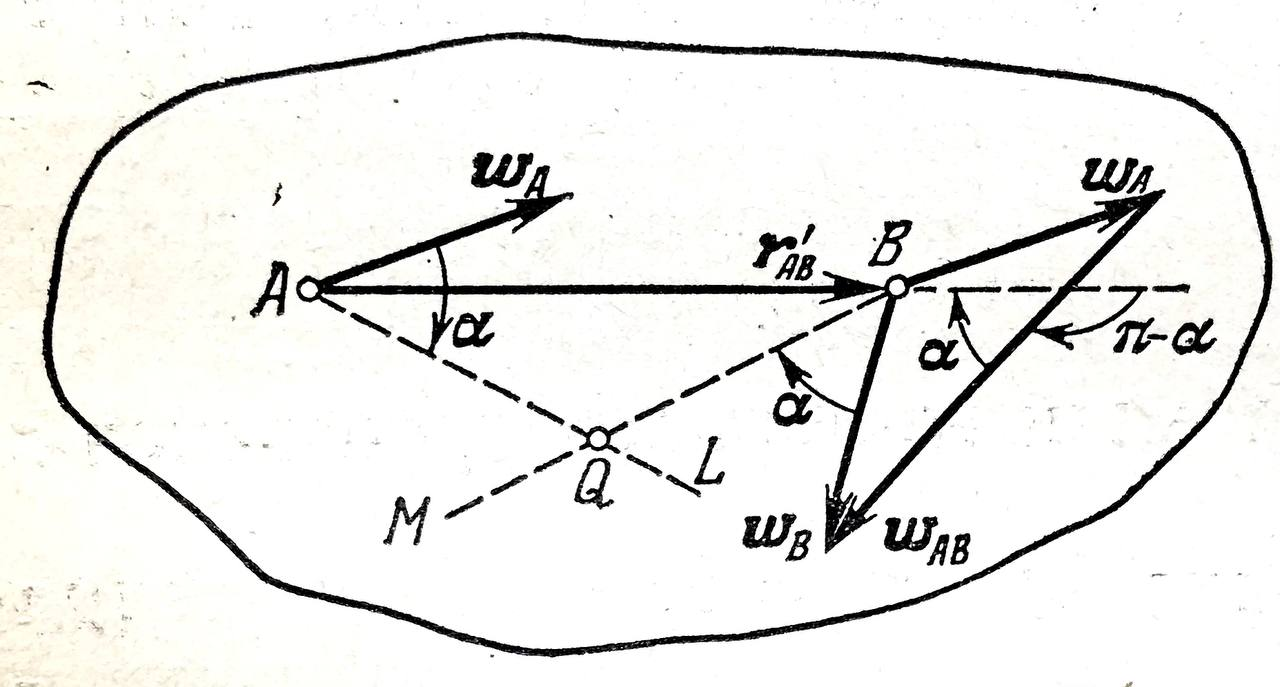
\includegraphics{src/mechanics/pictures/18_2.jpg}}

  \caption{}
  \label{fig:18_2}
\end{figure}

Построение мгновенного центра ускорений требует знания ускорения $\vec{w}_A$
какой-либо точки фигуры и угла $\alpha$. Покажем, как построить мгновенный
центр ускорений, имея ускорения двух точек фигуры. Заметим для этого, что, зная
$\vec{w}_A$ и $\vec{w}_B$, тем самым можем определить
\begin{equation*}
  \vec{w}_{AB} = \vec{w}_B - \vec{w}_A,
\end{equation*}
и, следовательно, угол $\alpha$ будет вполне определён. Теперь можем построить
луч $AL$, на котором лежит мгновенный центр ускорений $Q$. Нет надобности
вычислять положение точки $Q$ по формуле
\ref{eq:instantaneous_acceleration_center_distance}, так как можно построить её
графически, проведя ещё луч $BM$ под углом $\alpha$ к $\vec{w}_B$. Пересечение
лучей $AL$ и $BM$ определит точку $Q$.

Имея мгновенный центр ускорений, получаем весьма наглядную картину распределения
ускорений в плоской фигуре. Действительно, применяя формулу
\ref{eq:flat_motion_acceleration_named} в предположении, что за полюс $A$ принят
мгновенный центр ускорений $Q$, и замечая, что по определению $\vec{w}_Q = 0$,
получим
\begin{equation*}
  \vec{w}_B = \vec{w}_{QB} = \vec{w}_{QB}^\text{(в)} + \vec{w}_{QB}^\text{(ос)}
    = \crossprod{\vec{\varepsilon}}{\pvec{r}_{QB}} - \omega^2 \pvec{r}_{QB}.
\end{equation*}

Вращательное ускорение $\vec{w}_{QB}^\text{(в)}$ направлено по перпендикуляру к
вектор-радиусу, соединяющему центр ускорений с рассматриваемой точкой, в ту
сторону, куда происходит вращение, или в противоположную, смотря по тому,
является ли вращение ускоренным или замедленным.

Осестремительное ускорение $\vec{w}_{QB}^\text{(ос)}$ направлено всегда от точки
к мгновенному центру ускорений.

\begin{figure}[H]
  \centering
  \resizebox{\linewidth}{!}{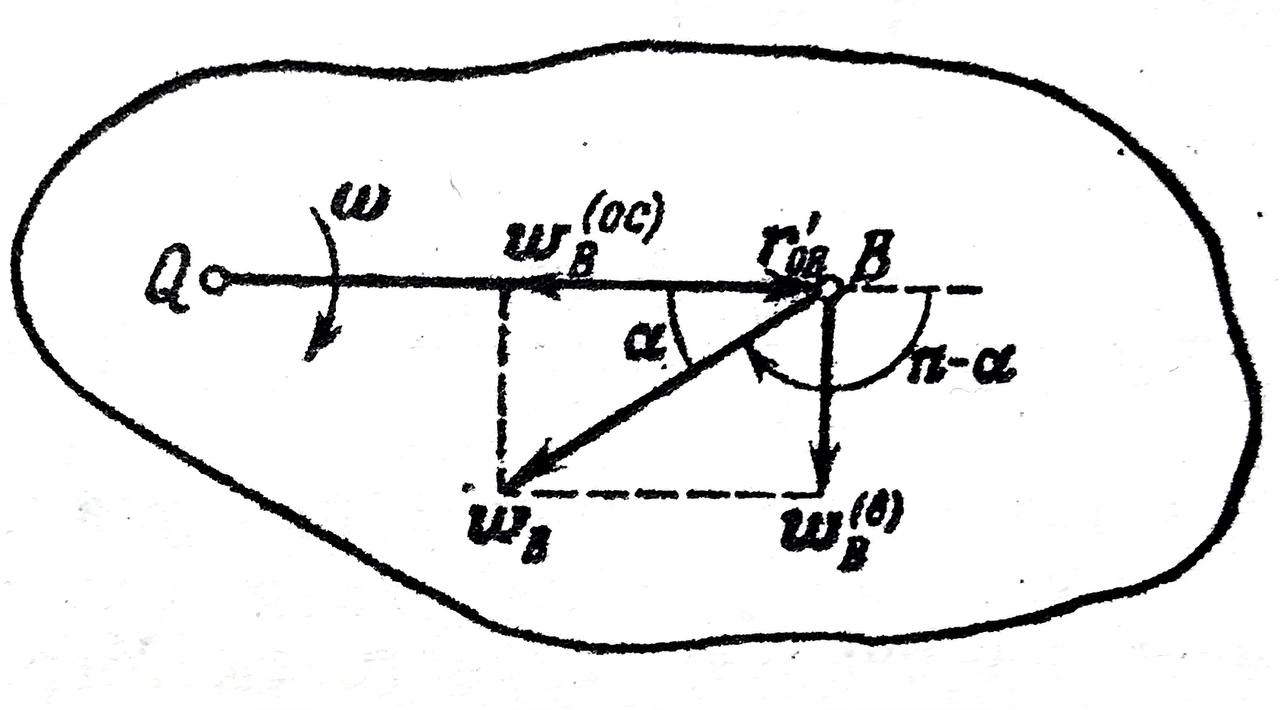
\includegraphics{src/mechanics/pictures/18_3.jpg}}

  \caption{}
  \label{fig:18_3}
\end{figure}

По величине они равны
\begin{equation*}
  \begin{gathered}
    w_{QB}^\text{(в)} = w_B^\text{(в)} = \varepsilon r_{QB}', \\
    w_{QB}^\text{(ос)} = w_B^\text{(ос)} = \omega^2 r_{QB}'.
  \end{gathered}
\end{equation*}
Их геометрическая сумма $\vec{w}_B$ по величине равна
\begin{equation*}
  w_B = r_{QB}' \sqrt{\varepsilon^2 + \omega^4}.
\end{equation*}

Таким образом, полное ускорение любой точки фигуры по величине пропорционально
её расстоянию от мгновенного центра ускорений и направлено под одинаковым для
всех точек фигуры углом к вектор-радиусу, соединяющему рассматриваемую точку с
мгновенным центром ускорений.

Не следует смешивать вращательное ускорение $\vec{w}_B^\text{(в)}$ с касательной
составляющей ускорения, а осестремительное ускорение $\vec{w}_B^\text{(ос)}$ ---
с нормальной составляющей. В самом деле, касательное $\vec{w}_\tau$ и нормальное
$\vec{w}_n$ ускорения направлены по касательной и главной нормали к
\textit{траектории}, то есть по перпендикуляру к вектор-радиусу $\pvec{r}_{PB}$,
соединяющему рассматриваемую точку с мгновенным центром скоростей $P$, и вдоль
этого вектор-радиуса, в то время как $\vec{w}_B^\text{(в)}$ и
$\vec{w}_B^\text{(ос)}$ направлены перпендикулярно и вдоль вектор-радиуса
$\pvec{r}_{QB}$.

\begin{figure}[H]
  \centering
  \resizebox{\linewidth}{!}{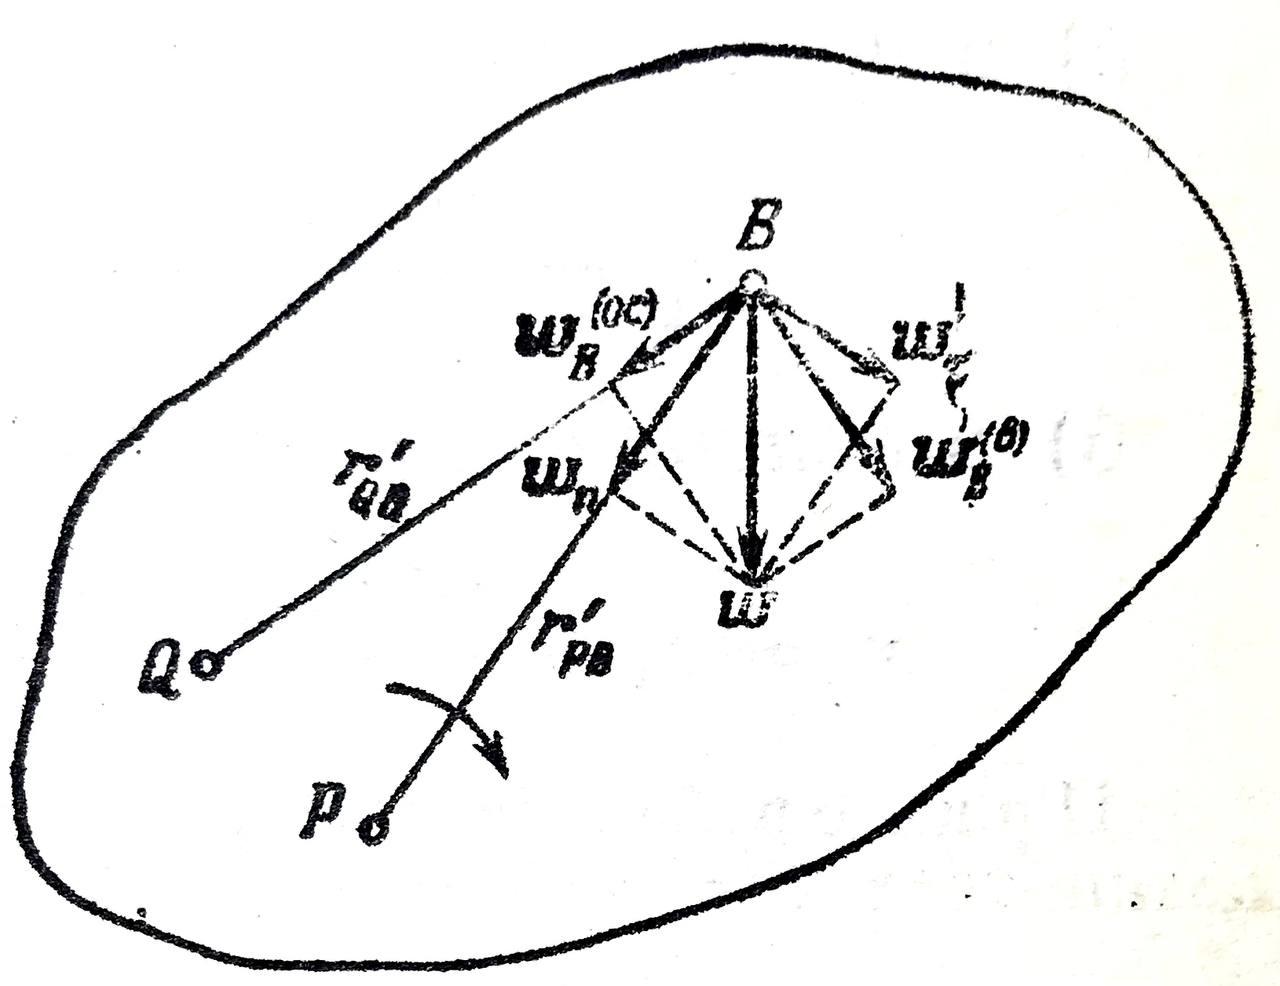
\includegraphics{src/mechanics/pictures/18_4.jpg}}

  \caption{}
  \label{fig:18_4}
\end{figure}

Легко получить вектор-радиусы $\vec{r}_Q$ и $\pvec{r}_Q$ центра ускорения в
неподвижной и подвижной системах координат; для этого решим векторное уравнение
\begin{equation}
  \label{eq:instantaneous_acceleration_center_acceleration}
  \vec{w}_Q = \vec{w}_0 + \crossprod{\vec{\varepsilon}}{\pvec{r}_Q} - \omega^2
    \pvec{r}_Q = 0.
\end{equation}
С этой целью умножим его векторно на $\vec{\varepsilon}$:
\begin{equation*}
  \crossprod{\vec{\varepsilon}}{\vec{w}_0} + \crossprod{\vec{\varepsilon}}
    {\crossprod{\vec{\varepsilon}}{\pvec{r}_Q}} - \omega^2 \paren{
      \crossprod{\vec{\varepsilon}}{\pvec{r}_Q} } = 0
\end{equation*}
и раскроем двойное векторное произведение; тогда получим
\begin{equation*}
  \crossprod{\vec{\varepsilon}}{\vec{w}_0} + \vec{\varepsilon} \paren{
    \dotprod{\vec{\varepsilon}}{\pvec{r}_Q} } - \pvec{r}_Q \paren{
    \dotprod{\vec{\varepsilon}}{\vec{\varepsilon}} } - \omega^2 \paren{
    \crossprod{\vec{\varepsilon}}{\pvec{r}_Q} } = 0.
\end{equation*}
Заметим, что в плоском движении $\dotprod{\vec{\varepsilon}}{\pvec{r}_Q} = 0$;
далее, из \ref{eq:instantaneous_acceleration_center_acceleration} следует, что
\begin{equation*}
  \crossprod{\vec{\varepsilon}}{\pvec{r}_Q} = \omega^2 \pvec{r}_Q - \vec{w}_0.
\end{equation*}
Окончательно получаем
\begin{equation*}
  \crossprod{\vec{\varepsilon}}{\vec{w}_0} - (\varepsilon^2 + \omega^4)
    \pvec{r}_Q + \omega^2 \vec{w}_0 = 0,
\end{equation*}
или, разрешая уравнение относительно $\pvec{r}_Q$,
\begin{equation*}
  \begin{aligned}
    \pvec{r}_Q &= \frac
      {\crossprod{\vec{\varepsilon}}{\vec{w}_0} + \omega^2 \vec{w}_0}
      {\varepsilon^2 + \omega^4} \\
    \vec{r}_Q &= \vec{r}_0 + \pvec{r}_Q =
      \vec{r}_0 + \frac
      {\crossprod{\vec{\varepsilon}}{\vec{w}_0} + \omega^2 \vec{w}_0}
      {\varepsilon^2 + \omega^4}.
  \end{aligned}
\end{equation*}

Проектируя первое равенство на подвижные оси координат $x',~y'$, а второе --- на
неподвижные оси $x,~y$, получим формулы координат мгновенного центра ускорений
$Q$:
\begin{enumerate}
  \item в \textit{подвижной} системе осей
    \begin{equation}
      \label{eq:instantaneous_acceleration_center_movable_coords}
      \begin{gathered}
        x_Q' = \frac
          {\omega^2 w_{0x'} - \ddot{\varphi} w_{0y'}}
          {\ddot{\varphi}^2 + \omega^4}, \\
        y_Q' = \frac
          {\omega^2 w_{0y'} + \ddot{\varphi} w_{0x'}}
          {\ddot{\varphi}^2 + \omega^4};
      \end{gathered}
    \end{equation}

  \item в \textit{неподвижной} системе осей
    \begin{equation}
      \label{eq:instantaneous_acceleration_center_immovable_coords}
      \begin{gathered}
        x_Q = x_0 + \frac
          {\omega^2 w_{0x} - \ddot{\varphi} w_{0y}}
          {\ddot{\varphi}^2 + \omega^4}, \\
        y_Q = y_0 + \frac
          {\omega^2 w_{0y} + \ddot{\varphi} w_{0x}}
          {\ddot{\varphi}^2 + \omega^4}.
      \end{gathered}
    \end{equation}
\end{enumerate}

\subsection{Список литературы}
\begin{enumerate}
  \item \cite{lourie}
\end{enumerate}

